\chapter{Benefits and costs of an incomplete degree} \label{chap:2}

Policy concern about dropping out is driven by concern about its cost. Students spend time and money on study that does not deliver the benefits of a completed degree. Most people who drop out of university report some benefits, including improved skills and employment, interest in what they studied, and making friends. Nearly half of them would still begin their degree, knowing what they know now. For people who are unsure of their direction, there is a benefit in exploring higher education as one of their options.

But there are also costs. Most people who leave without a degree have HELP debts below \$10,000. But some drop out with substantial debts after years of study. Almost one-in-five people who drop out say they received no benefits at all from their time at university.

Most people who dropped out believe that they would be better off if they had a degree.

\section{Student perceptions}\label{sec:2.1}

Trying university can have benefits even for students who do not complete a degree. A Grattan Institute online survey of people with an incomplete degree suggests that for many the benefits outweigh the costs.\footnote{The survey was conducted between late 2017 and early 2018, see \Chapref{chap:b} for more detail.} More than 40 per cent of respondents said that, knowing what they know now, they would still have begun their degree (\Cref{fig:6}). Remarkably, of this group, nearly half would still leave. Even though they did not finish their course, enrolling brought benefits.

But the survey also shows that almost 40 per cent of people who did not complete would not have started their degree, knowing what they know now. Although their time at university might have brought some benefits, the costs were greater and, with the benefit of hindsight, they would not have attended.

                % Figure 6
                \begin{figure}
                    \caption{Many people who drop out would still begin the degree, knowing what they know now\label{fig:6}}%
                    \units{Per cent}
                    \includegraphics[page=9]{atlas/selection_chartdeck.pdf} 
                    \noteswithsource{Only includes students who have never completed a degree, 376 respondents.}
                    {Grattan survey of people with an incomplete university degree, 2017-18. See \Chapref{chap:b} for details.}
                \end{figure}


\subsection{Time and student contribution costs}\label{subsec:2.1.1}

The time and money costs of incomplete degrees vary significantly. Many students leave quickly during the mutual selection process (\Cref{sec:1.1}). They haven't necessarily spent much time studying. Using the 2008 commencing cohort as an example, more than half of the students who did not complete took the equivalent of a year's worth of subjects or less (\Cref{fig:7}). Nearly a third of students who dropped out took the equivalent of one full-time semester or less (the calendar time would be longer for part-time students). With universities typically recommending about 10 hours each week per subject for attending classes and private study, a student would spend about 600 hours studying to complete a semester. In practice, many students who drop out probably spend less time than this engaged in academic activity (\Cref{sec:6.2}).

As \Cref{fig:7} shows, older students take fewer subjects before leaving. Almost half of students who commenced after turning 30 and dropped out did so having taken half a year of subjects or less. By comparison, less than 20 per cent of school-leaver entrants left having taken half a year of subjects or less.

Students pay for their education by subject, so if they leave quickly the financial costs are kept down. \Vref{fig:8} uses historical completion statistics to estimate the contributions of bachelor-degree students who commenced in 2017 and are not expected to complete their course. Almost a third of them are expected to pay or borrow less than \$5,000, and more than half are expected to incur total costs below \$10,000.


                % Figure 7
                \begin{figure}
                    \caption{Older students leave more quickly\label{fig:7}}%
                    \units{Proportion of students by subjects taken before dropping out, per cent}
                    \includegraphics[page=10]{atlas/selection_chartdeck.pdf} 
                    \noteswithsource{Drop out refers to people who have not completed a bachelor degree and were not enrolled in their 7\textsuperscript{th}~or 8\textsuperscript{th}~year. The analysis is based on domestic bachelor degree students~who commenced in 2008.}
                    {Grattan analysis of \textcite{DepartmentofEducationandTraininga}}
                \end{figure}




Not all these students will repay. From 2018-19, HELP debtors make repayments only in years when they earn about \$52,000 or more.\footnote{Unless the HELP repayment income threshold is lowered to \$45,000, as the government proposes: \textcite{AustralianGovernment2017b}.} So some students who drop out will not repay any of their debt, or repay only part of what they borrowed.

For the students who do repay, \$10,000 or less in student contribution costs is unlikely to make their lifetime financial position dramatically worse. Nevertheless, if they received few or no benefits from their study this is money they could have better spent on something else.

Although most students who drop out spend less than \$10,000 and modest amounts of time, some invest much more than this without getting a degree. Ten per cent spend the equivalent of three or more years of full-time study before departing. Eight per cent end up owing \$30,000 or more. On average, students who drop out borrow \$12,000.

\subsection{Career costs and benefits }\label{sec:2.1.2}

The main long-term cost of not finishing a course is lost labour market opportunities. Most students have job and career reasons in mind when they enrol in university.\footcites[][24]{Baik2015}[][chapter~5]{Long2006} 
Without their degree, students may miss out on a career they wanted, and the additional lifetime earnings that, on average, graduates receive.\footcites[][]{Norton2012}[][]{Borland2000}[][]{Wei2010}[][]{Daly2012}

                % Figure 8
                \begin{figure}
                    \caption{Most students who drop out will pay or borrow less than \$10,000\label{fig:8}}%
                    \units{Per cent of students by debt level (\$2017)}
                    \includegraphics[page=11]{atlas/selection_chartdeck.pdf} 
                    \noteswithsource{Student contributions are calculated using the six-digit field of education code and 2017 funding rates. Twelve per cent of student contributions were paid upfront. See also \Cref{fig:7}}
                    {Grattan analysis of \textcite{DepartmentofEducationandTraining2017g} and \textcite{DepartmentofEducationandTraininga}}
                \end{figure}


In theory, people who start but do not finish university should have higher average incomes than people who never went to university, but lower than graduates. Admission to higher education suggests above-average cognitive ability, and university students may acquire knowledge and skills with labour market value without completing their course. These factors should boost pay, on average. But people who leave university without a degree lack skills or credentials required or preferred in many high-paying occupations, limiting their career opportunities.\footnote{\textcite{Schnepf2017}, using European data, provides empirical support for the theory.}

The Grattan online survey of people who had started but not finished a degree allows us to explore the idea that students acquire employment benefits from incomplete degrees. Of the people who said they would still begin their degree, despite knowing that they will not complete, many reported significant employment-related benefits from their incomplete degree, as \Cref{fig:9} shows. Of this group, more than 60 per cent said that their course `taught them useful skills', one-third said it `helped clarify career goals', and one-quarter reported that their incomplete degree `helped them get employed'. The people who would not begin their degree again also reported some employment-related benefits, but at lower levels than those who would begin their degree again. These results are consistent with a recent single-university survey, which found that nearly half of students who left without completing see their study as helpful for their career goals.\footcite[][37]{Harvey2017a}


                % Figure 9
                \begin{figure}
                    \caption{Students who don't complete report benefits from their time at university\label{fig:9}}%
                    \units{``Were there any benefits from the time you spent doing the incomplete degree?'', per cent}
                    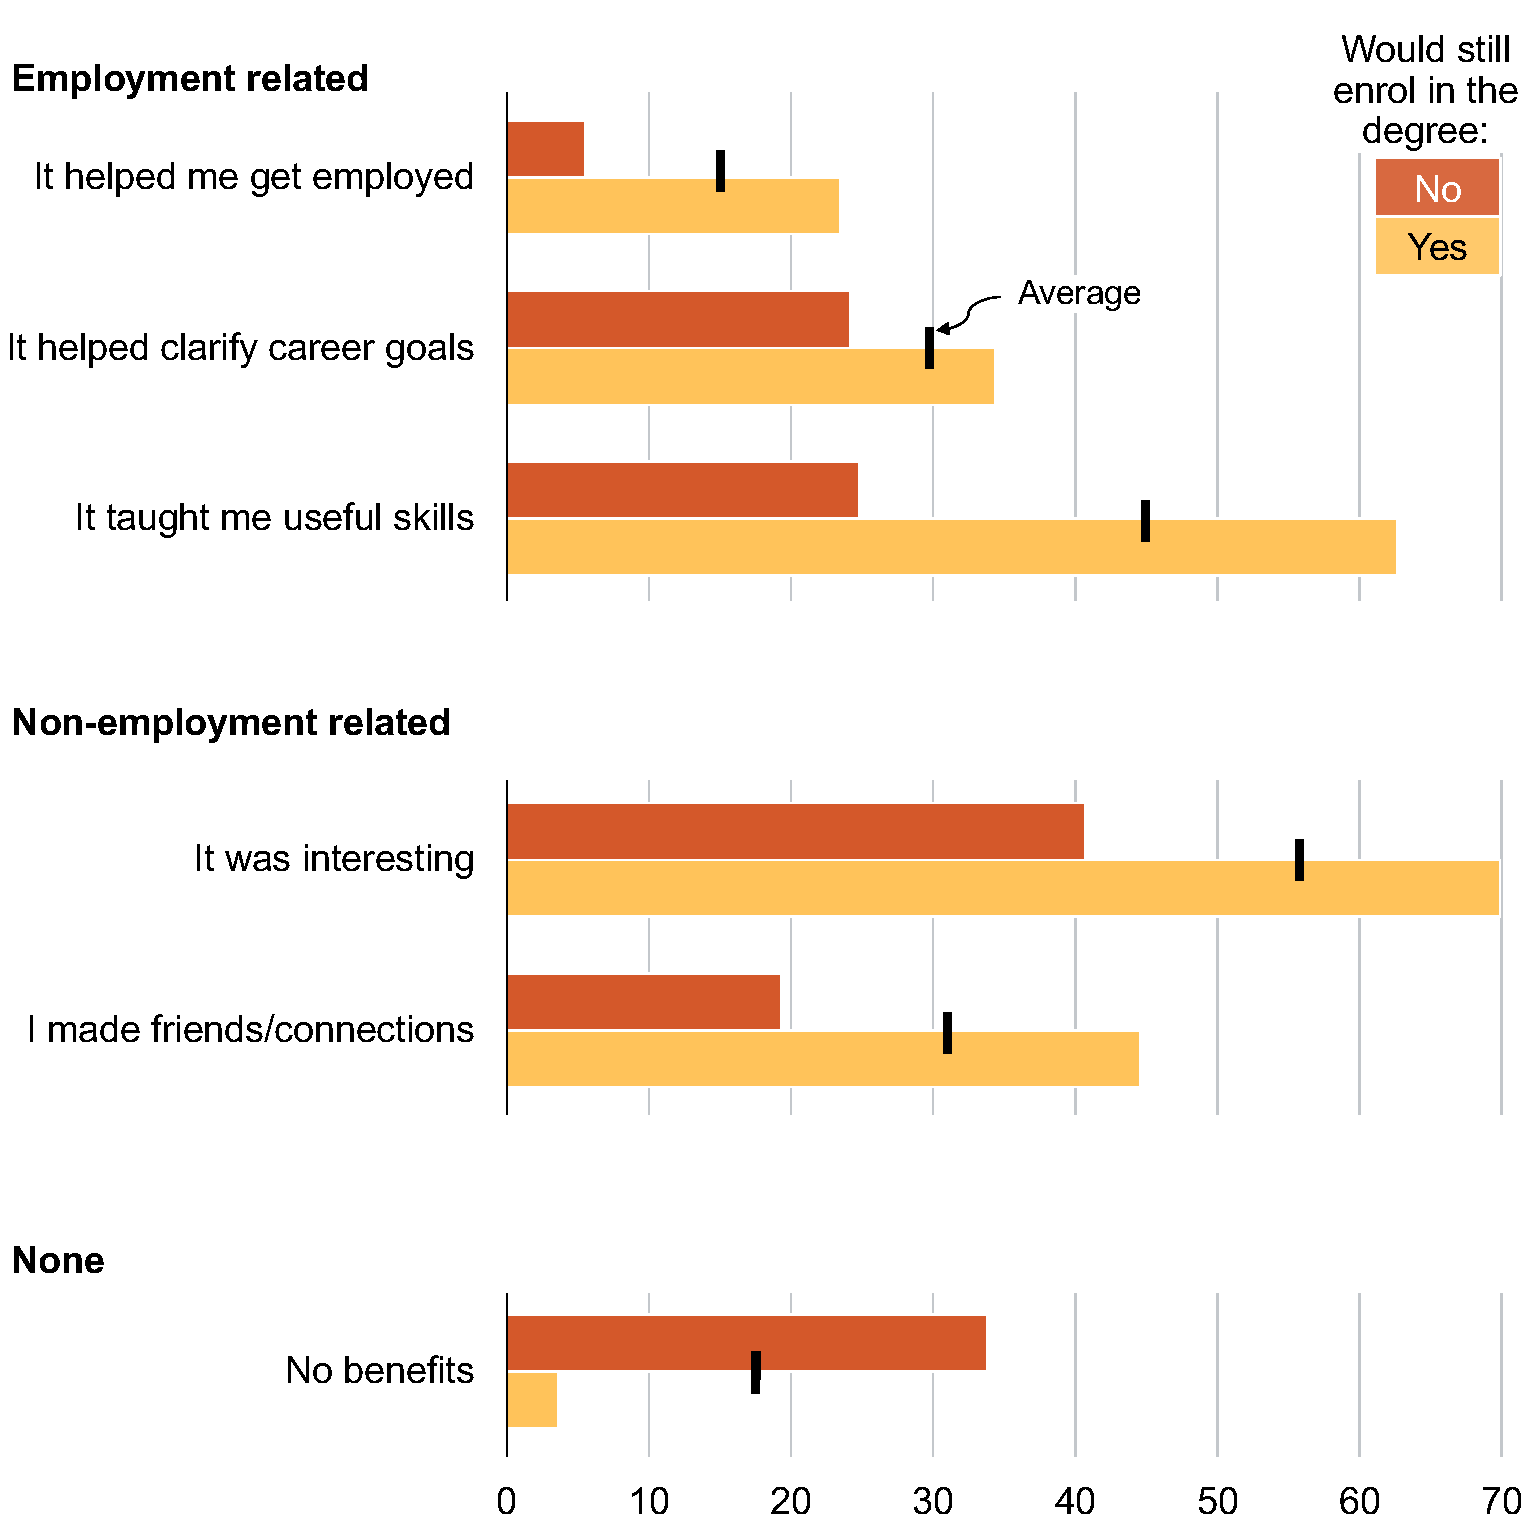
\includegraphics[page=1]{atlas/benefits_halfpage.pdf} 
                    \noteswithsource{Only includes 311 respondents who dropped out and do not hold a bachelor degree.}
                    {Grattan survey of people with an incomplete university degree, 2017-18.}
                \end{figure}


The career benefits of incomplete qualifications are reflected in earnings. \Cref{fig:10} shows that people who start a degree earn considerably more than people who never enrolled, but also less than people who complete their degree. The median annual income of people with an incomplete bachelor degree and no other post-school qualification is close to \$12,000 more than someone with Year 12 but no further study. But it is about \$15,000 below that of someone who completed their bachelor degree.

At the median, a diploma-holder who attempted a bachelor degree earns nearly \$14,000 a year more than one who did not. This is consistent with diploma-holders who were admitted to a bachelor degree being more able and skilled than other diploma-holders, with some of their skills potentially learned while enrolled in their bachelor degree.

\Cref{fig:10} also shows that, at the median, someone with an incomplete bachelor degree but with a Certificate III/IV or a diploma or advanced diploma earns only moderately less than someone with a bachelor degree. Almost half of people with an incomplete bachelor degree have one of these qualifications.\footnote{Excluding people who completed another bachelor degree or above, \textcite{ABS2016f}.}

This positive earnings information on diplomas needs a caveat. ABS surveys and other data sources suggest that upper-level vocational qualifications benefit men more than women, at least financially. As \Vref{fig:11} shows, early-career women with these qualifications earn much the same as women who finished their education at Year 12.\footcites[][49--51]{Wilkins2016}[][section~3.2.2]{Norton2017d} 
This suggests that women who drop out of university forgo more earnings than men.

                % Figure 10
                \begin{figure}
                    \caption{People who begin a bachelor degree generally earn more, even if they don't complete\label{fig:10}}%
                    \units{Median annual earnings from all sources all ages, \$2015}
                    \includegraphics[page=13]{atlas/selection_chartdeck.pdf} 
                    \noteswithsource{`Diploma' also includes advanced diploma. Excludes people who were studying at any level. `Did not start uni' represents those with no incomplete bachelor-or-above courses. `Dropped out' group is composed of those whose highest incomplete qualification is a bachelor degree. `Bachelor' includes those with an incomplete qualification, provided they have completed at least one bachelor degree. Includes people who are not working.}
                    {\textcite{ABS2016f}}
                \end{figure}

                % Figure 11
                \begin{figure}
                    \caption{Women gain little financial benefit from upper-level vocational qualifications\label{fig:11}}%
                    \units{Median annual income from all jobs, 25-to-34 years old in 2016, \$}
                    \includegraphics[page=14]{atlas/selection_chartdeck.pdf} 
                    \noteswithsource{Sample includes people born in Australia or born overseas and arrived in Australia at least ten years ago, employed and not studying. Weighted by weekly earnings in all jobs. The income differences are larger than they appear in \Cref{fig:10} because it includes people who are not working.}
                    {\textcite{ABS2017f}}
                \end{figure}


\subsection{Non-financial costs and benefits}\label{subsec:2.1.3}

Although most commencing students have career goals, students overwhelmingly choose courses that interest them. Ninety-five per cent of first-year students agree that `studying in a field that really interests me' is an important reason for enrolling.\footcite[][24]{Baik2015} On this goal, higher education often delivers, even for those who do not complete. Among the people who would still enrol in a degree, 70 per cent found their incomplete course interesting, and even among people who would not have enrolled in hindsight, 40 per cent found their course interesting. (\Vref{fig:9}).

University is also a place to meet people and make friends. More than 40 per cent of the people who did not complete, but would still enrol in their degree anyway, made lasting friendships or connections while at university. But less than 20 per cent of the people who would not do their degree again made lasting friendships or connections at university.

Friendships contribute to well-being, but the broader psychological consequences of trying university are unclear. In recent surveys, younger university students report higher rates of psychological distress than non-students of the same age.\footcite[][]{Cvetkovski2012} 
Among students considering leaving without finishing, the single most commonly cited reason is `health or stress'.\footnote{The survey starts collecting data in second semester, so the data excludes students who left earlier, \textcite[][12]{SocialResearchCentre/DepartmentofEducationandTraining2017}. In the Grattan survey of people with incomplete degrees, 18 per cent of those who do not currently have a bachelor degree gave a mental health reason for leaving university.} 
For some students, concluding that enrolment was a mistake, or struggling with academic work, may cause or exacerbate mental health problems.\footnote{One recent Australian study found an association between mental health issues, alcohol consumption and missing classes and not completing assignments: \textcite{Tembo2017}. However, another Australian study found, counter-intuitively, that people with anxiety or depression were not less likely to complete their degree: \textcite{Cvetkovski2018}.} If so, that may be a cost of attending university.

Dropping out may remove some triggers for mental health problems. But it may not resolve all psychological issues. In the Grattan survey of people with incomplete degrees, more than two-thirds of respondents felt that by dropping out they had let themselves or someone else down (they may also have felt this if they had not attended in the first place).\footnote{More than half of respondents who did not have a degree felt they had let their family down.} 
In an ABS survey, people with an incomplete bachelor degree were twice as likely to report a long-term mental health condition as people with bachelor degrees who had never dropped out.\footnote{\textcite{ABS2016f}. This was true whether or not they subsequently went on to complete a degree.} However, we do not know whether or to what extent these mental health issues are linked to their university experience.


\subsection{Selection costs and benefits }\label{subsec:2.1.4}

The long mutual selection process described in \Cref{sec:1.1} has benefits. A selection system with low application fees and a lengthy try-before-you-buy period lowers the risk of going to university. People are more prepared to apply and enrol if the costs of enrolment are low. Even if the motive for attending university is to comply with parental desires or to join friends, some may discover that it is interesting and they want to continue. Their careers and lifetime earnings could be substantially better as a result.

Subsequent chapters will suggest improvements to the mutual selection process. But even with these changes there will still be many things that applicants don't know about themselves and about university, and many things that universities don't know about applicants. This uncertainty means that, to some extent, incomplete degrees are an inevitable cost of seeking to match people with courses and careers. Although it is difficult to quantify the benefits to the people who might never have started under a different system, these should be considered along with the costs to students who start courses but do not finish.

For the students whose enrolment does not work out, the time and money spent experimenting with university are not necessarily wasted. Clarifying their course and career goals can be beneficial. So can making friends and learning things that are interesting or useful.

\section{Reducing costs and increasing benefits}\label{sec:2.2}

Most students who go to university report some benefits, whether they complete or not. But in some cases, the benefits could have been greater than they were. More than 60 per cent of the people who dropped out and have no other degree think that their position would be better if they had finished (\Vref{fig:12}). For some, this might be a general recognition that graduates usually earn more, not a belief that they should have tried harder to complete. But \Vref{fig:9} shows that around a quarter of those who would begin their degree again would not drop out if they had their time again. This points to some potential to improve completion rates, through better decisions by students and changes to university practices.

A third of the people who would not begin the degree again if they had their time again report no benefits at all; this is one in five of all respondents to the Grattan survey of people who do not currently have a degree. In their view, the time and money they spent at university did not deliver commensurate benefits. The following chapters discuss how we can identify these students more quickly, and how the selection system can better protect them from costly mistakes.


                % Figure 12
                \begin{figure}
                    \caption{Most people who don't complete their degree believe they would have been better off if they had completed\label{fig:12}}%
                    \units{``Do you think you would be in a better position now if you had finished your incomplete degree?'', per cent}
                    \includegraphics[page=15]{atlas/selection_chartdeck.pdf} 
                    \source{See \Cref{fig:6}}
                \end{figure}



